\subsection{Reference Implementation}
\label{subsec:referenceImpl}

Before implementing a code generator one has to know what the target code is. Therefore a reference implementation has been
developed which was coded to large degree manually. From this reference code the templates can be derived. Also this is a
manual step.
\begin{wrapfigure}[24]{l}{0.48\textwidth}
 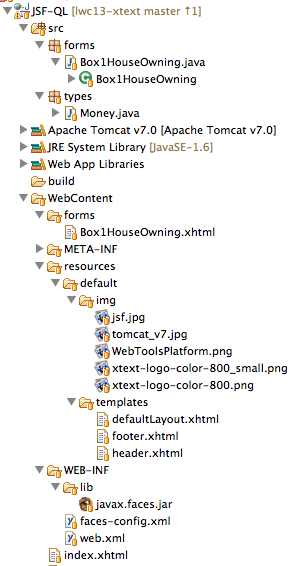
\includegraphics[width=9cm]{./images/chapter02/referenceimpl_projecttree.png}
\end{wrapfigure}
We use a Java Server Faces (JSF, see \ref{subsec:technologyStack}) based
application, which can be deployed on any Java Web container (also known as a Servlet container) like Glassfish, JBoss and Apache Tomcat.

The screenshot shows the structure of the web application project. The application is available for download from the project 
homepage (\href{http://lwc13-xtext.eclipselabs.org.codespot.com/files/JSF-QL-1.0.zip}{JSF-QL-1.0.zip})
 
Large parts of the application are not derivable from the model, they build the skeleton of the project. This is:
\begin{itemize}
\item Custom types (\texttt{src/types/*})
\item Custom type converter (\texttt{src/converter/*})
\item Libraries \newline (\texttt{WebContent/WEB-INF/lib/*})
\item Web Application Descriptor \newline (\texttt{WebContent/WEB-INF/web.xml})
\item Faces configuration \newline
(\texttt{WebContent/WEB-INF/faces-config.xml})
\item Images \newline (\texttt{WebContent/resources/default/img/*})
\item Page Templates \newline
(\texttt{WebContent/resources/default/templates/*})
\end{itemize} 

After describing some necessary configuration of the IDE we will focus on the
parts which are dependent on the QL model and thus subject of code generation
in sub sesction \ref{subsec:referenceForms}.
These artifacts are:
\begin{itemize}
\item Java Bean classes representing the state of a Form (\texttt{src/forms})
\item JSF enabled XHTML pages representing the presentation of a Form (\texttt{WebContent/forms/*})
\end{itemize}

\subsubsection{IDE Configuration}

\paragraph{Webtools}
install new software

http://download.eclipse.org/releases/juno/

Collaboration	
-     

Web, XML, Java EE and OSGi Enterprise Development	
\begin{itemize}
	\item Eclipse Java EE Developer Tools	3.4.0.v201107072300
	\item JavaServer Faces Tools (JSF) Project	3.4.1.v201208241503
	\item JST Server Adapters	3.2.200.v20120517\_1442
	\item JST Server UI	3.4.0.v20120503\_1042
	\item JST Server Adapters Extensions	3.3.101.v20120821\_1416
	\item Eclipse Web Developer Tools	3.4.1.v201208170345
	\item Eclipse Java Web Developer Tools	3.4.1.v201208231800
\end{itemize} 
\paragraph{Install Tomcat}

add new server:
- tomcat v7



\subsubsection{Import and run reference}

Checkout from git OR downlaod from project home page @ code.google.com

import project from git:
checkout instructions:
https://code.google.com/a/eclipselabs.org/p/lwc13-xtext/source/checkout

download zip from:
project home: http://code.google.com/a/eclipselabs.org/p/lwc13-xtext/

run as MWE2 Workflow

1. /org.eclipse.xtext.example.ql/src/org/eclipse/xtext/example/ql/GenerateQlDsl.mwe2

2. /org.eclipse.xtext.example.qls/src/org/eclipse/xtext/example/qls/GenerateQlsDsl.mwe2

Run configuration

- LWC13 Runtime

import existing project
- \\lwc13-xtext\\examples\\QLTest

\subsubsection{Main Layout}
\label{subsec:referenceMainLayout} 

The logical entry to the web application is the welcome file
\texttt{WebContent/index.xhtml} declared in
\texttt{WebContent/WEB-INF/web.xml}. The \texttt{index.xhtml} composes the
main layout with page contents and will later be helpful to integrate the
generated artifacts with the web application's layout by using JSF's XHTML
templating
\footnote{\url{http://docs.oracle.com/javaee/6/javaserverfaces/2.1/docs/vdldocs/facelets/}}.

\begin{lstlisting}[language=HTML]
<?xml version='1.0' encoding='UTF-8' ?>
<!DOCTYPE html PUBLIC "-//W3C//DTD XHTML 1.0 Transitional//EN" 
    "http://www.w3.org/TR/xhtml1/DTD/xhtml1-transitional.dtd">
<html xmlns="http://www.w3.org/1999/xhtml"
  xmlns:h="http://java.sun.com/jsf/html"
  xmlns:ui="http://java.sun.com/jsf/facelets">
<body>

  <ui:composition
    template="/resources/default/templates/defaultLayout.xhtml">
    <ui:define name="content">
      Hello World!
    </ui:define>
  </ui:composition>

</body>
</html>
\end{lstlisting}
 
Subpages of the application should use the \texttt{index.xhtml} placed in
\texttt{WebContent/} itself as their template and overwrite the content section
with custom output via the same pattern.

\begin{lstlisting}[language=HTML] 
	<ui:composition template="/index.xhtml">
  		<ui:define name="content">
  		...my xhtml content
  		</ui:define>
 	</ui:composition>
\end{lstlisting}

Everything between the opening and closing \texttt{facelet:define} tag within
the subpage will be passed into a corresponding \texttt{facelet:insert} section
(\texttt{name} attribute is set to \texttt{''content''}) defined in the template
(here: \texttt{defaultLayout.xhtml}) or one of its parent templates when the HTML output is rendered by the JSF framework.

\subsubsection*{Default template}
\label{sec:template}

We keep the main layout definition and the page contents separated from each
other. The \texttt{WebContent/index.xhtml} defines the main composition of the
application's structural layout and content of pages as described in section
\ref{subsec:referenceMainLayout}. Layout template defintions should be placed in
a folder \texttt{WebContent/resources/*templateName*} in our web
application.

To change the main layout it is just necessary to change the \texttt{template}
reference of the \newline\texttt{facelets:composite} in
\texttt{WebContent/index.xhtml}.\newline

\begin{lstlisting}[language=HTML]
 ...
  <ui:composition
    template="/resources/default/templates/defaultLayout.xhtml">
 ...
\end{lstlisting}

The reference application is shipped with a default template placed in \newline
\texttt{WebContent/resources/default/}. It is a very simple one
providing only a skeleton \newline \texttt{/templates/defaultLayout.xhtml} with
basically 3 sections (header, content, footer) where clients can add custom
content.

The current web application expects a defined \texttt{facelets:insert}
section with name 'content' within the template or one of its parents for proper
composition. In our reference implementation it is declared in
\texttt{/resources/default/templates/defaultLayout.xhtml}.

\begin{lstlisting}[language=HTML]
<!DOCTYPE html PUBLIC "-//W3C//DTD XHTML 1.0 Transitional//EN" 
          "http://www.w3.org/TR/xhtml1/DTD/xhtml1-transitional.dtd">
<html xmlns="http://www.w3.org/1999/xhtml"
	xmlns:h="http://java.sun.com/jsf/html"
	xmlns:ui="http://java.sun.com/jsf/facelets">
<h:head>
	<title><ui:insert name="title">LWC 2013 Xtext</ui:insert></title>
</h:head>
<body>
	<div id="header">
		<ui:insert name="header">
			<ui:include src="/resources/default/templates/header.xhtml" />
		</ui:insert>
	</div>
	<div id="content">
		<ui:insert name="content">
    	Content area. Compose by use of tag facelet:define & name="content".
  </ui:insert>
	</div>
	<div id="footer">
		<ui:insert name="footer">
			<ui:include src="/resources/default/templates/footer.xhtml" />
		</ui:insert>
	</div>
</body>
</html>
\end{lstlisting}

We added two \texttt{facelets:insert} sections to give the possibility to
replace the header and footer. To simplify the concrete JSF compositions later we let JSF include
default content for both by use of \texttt{facelets:include} for a fixed source
\texttt{src}.

Our structural layout definition which is composed by using
\newline\texttt{/resources/default/templates/defaultLayout.xhtml} as template in
\newline \texttt{WebContent/resources/default/} has a Cascading Style Sheet (CSS)
\footnote{\url{http://de.wikipedia.org/wiki/Cascading_Style_Sheets}} where fine
grained layouting can be done.

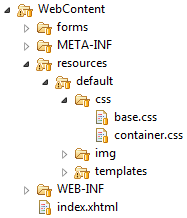
\includegraphics{./images/chapter02/css_template.png}

The applications style sheets consist of 2 files.

\begin{itemize}
\item \texttt{container.css} - defines styles for main page elements, basically we took
the style of \url{http://www.itemis.de/}
\item \texttt{base.css} - defines extended elements like grids,see
\url{http://www.yaml.de/docs/}
\end{itemize} 

Because we are not focusing on main layout topics, we just did some simple
things to integrate the style with the contents like adding CSS classes to XHTML elements.
The CSS definitions are added to show how dividing of content and styles
can be done.


\subsubsection{Reference Forms}
\label{subsec:referenceForms}
general (eg dependency baseForm, form)

\paragraph{Bean}
yxcvyxcvyxcvyxcvyxcv

\paragraph{Form}
yxcvyxcvyxcvyxcvxycv



